\documentclass{article}
\title{\sc Bombo Batidor/Mezclador para Cofitería.}
\author{\it Erick I. Rodríguez Juárez.}
\usepackage[margin = 0.5in]{geometry}
\usepackage{graphicx}
\usepackage{amsmath}
\begin{document}
\maketitle

\section{\centering --- Variables ---} % (((
Se definen:
\begin{center}
  \begin{tabular}{|l|l|l|}
    \hline 
    Variable & Descripción   & Unidades\\ \hline 
    Y:  & Precio del activo  & MXN \\ \hline 
    X1: & Edad del activo    & Años \\ \hline 
		X2: & Volumen  & \(m ^ 3\) \\ \hline 
  \end{tabular}
\end{center} 
% )))

\section{\centering --- Datos Usados ---} % (((
Se toma una muestra estadísticamente significativa. \\ 
La comprobación de este hecho se realiza la comprobación de este hecho a lo largo de las siguientes secciones.
\begin{center}
	\begin{tabular}{*{4}{|p{2cm}}|}
		\hline 
MARCA    & EDAD  & VOL  & PRECIO \\ \hline
COMFIT   & 0     & 2.7  & \$38,9971.12 \\ \hline
Sin Dato & 0     & 2.7  & \$36,6545.35 \\ \hline
CBA4     & 50    & 2.7  & \$14,0803.50 \\ \hline
CP4      & 34    & 3.2  & \$21,8300.00 \\ \hline
	\end{tabular}
\end{center}
% )))

\section{\centering --- Matriz de Dispersion ---} % (((
\begin{center}
  \begin{tabular}{|p{11cm}|p{5cm}|}
    \hline
    Gráfica & Interpretación. \\ \hline 
    \begin{minipage}{\textwidth}
    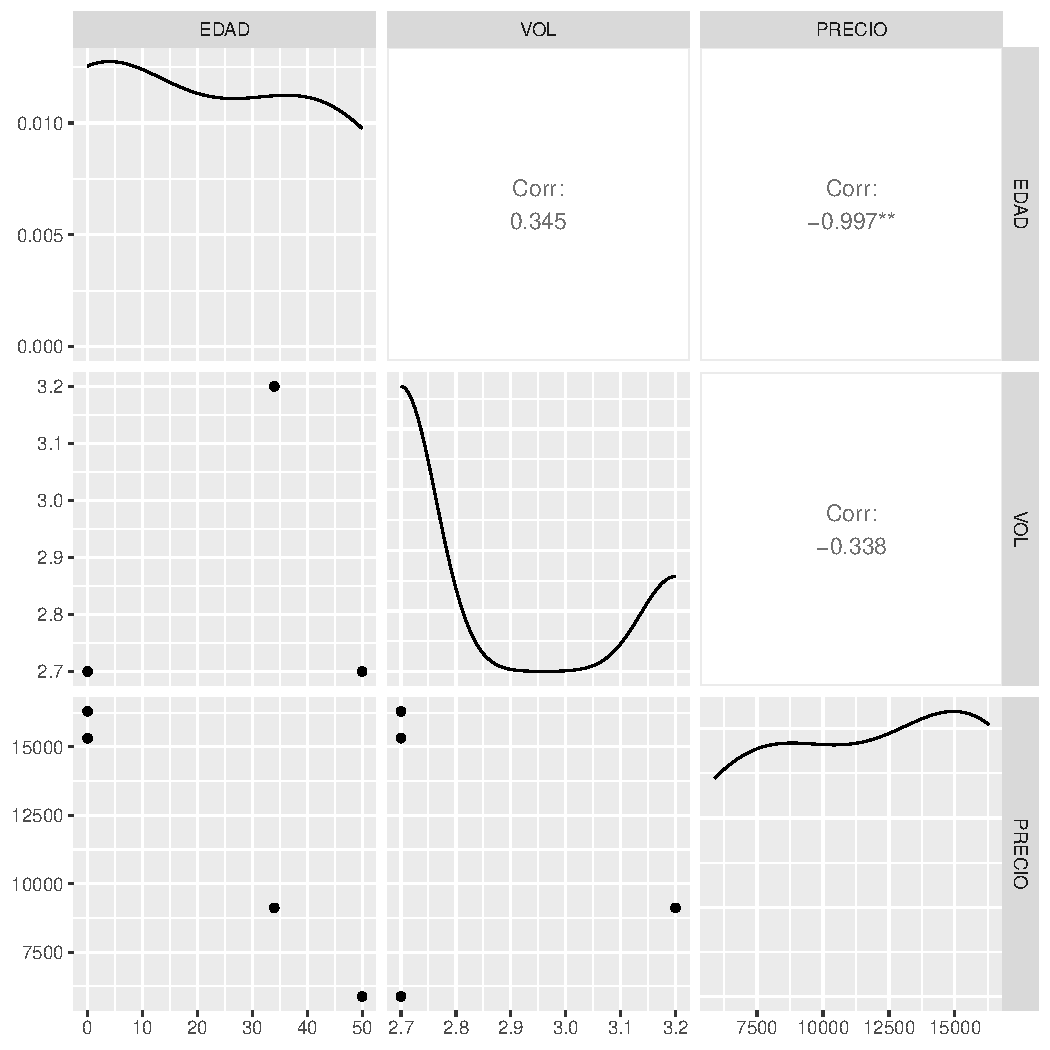
\includegraphics[width= 0.5 \linewidth, page=1]{r/Rplots.pdf}
    \end{minipage} 
    &
		Se tiene una correlación lineal negativa fuerte (el \(99.7\%\) de los datos lo corroboran),
		entre la Edad del Activo, y el Precio del Activo.
		\\ \hline 
  \end{tabular}
\end{center} 
% )))

\newpage

\section{\centering --- Supuestos del Modelo de Regresión ---} % (((

Se realizará el análisis estadístico con un \(90\%\) de confianza. \\ 
Es decir, \(1- \alpha = 0.9\).

\subsection{--- Homocedasticidad ---} % (((
\begin{center}
  \begin{tabular}{|l|p{8cm}|}
    \cline{1-2}
    \multicolumn{2}{|c|}{Hipótesis}\\ \cline{1-2}
    \multicolumn{2}{|l|}{\(H_0:\) La varianza de los residuales es constante.} \\ 
    \multicolumn{2}{|l|}{\(H_a:\) La varianza de los residuales no es constante.} \\ \cline{1-2}
    Estadístico de Prueba & \(BP = 4\).\\ \cline{1-2} 
		Región de Rechazo de \(H_0\) & \((0, \alpha )\).\\ \cline{1-2} 
    Valor \(p\) & \(0.1353\).\\ \cline{1-2} 
    Conclusión & Se tiene que \(p> \alpha\). \newline 
		Por tanto no se rechaza \(H_0\). \newline 
		Es decir, la varianza no es constante. \\ \cline{1-2} 
  \end{tabular}
\end{center}
% )))

\subsection{--- Independencia ---} % (((
\begin{center}
  \begin{tabular}{|l|p{8cm}|}
    \cline{1-2}
    \multicolumn{2}{|c|}{Hipótesis}\\ \cline{1-2}
    \multicolumn{2}{|l|}{\(H_0:\) Los residuos son independientes.} \\ 
    \multicolumn{2}{|l|}{\(H_a:\) Los residuos no son indpendientes.} \\ \cline{1-2}
    Estadístico de Prueba & \(DW = 2.5\).\\ \cline{1-2} 
		Región de Rechazo de \(H_0\) & \((0, \alpha )\).\\ \cline{1-2} 
    Valor \(p\) & \(1\).\\ \cline{1-2} 
    Conclusión & Se tiene que \(p> \alpha\). \newline 
		Por tanto no se rechaza \(H_0\). \newline 
		Es decir, los residuos son independientes.\\ \cline{1-2} 
  \end{tabular}
\end{center}
% )))

\subsection{--- Normalidad ---} % (((
\begin{center}
  \begin{tabular}{|l|p{8cm}|}
    \cline{1-2}
    \multicolumn{2}{|c|}{Hipótesis}\\ \cline{1-2}
    \multicolumn{2}{|l|}{\(H_0:\) Los residuos siguen una distribución normal} \\ 
    \multicolumn{2}{|l|}{\(H_a:\) Los residuos no siguen una distribución normal.} \\ \cline{1-2}
    Estadístico de Prueba & \(W = 0.94466\).\\ \cline{1-2} 
		Región de Rechazo de \(H_0\) & \((0, \alpha )\).\\ \cline{1-2} 
    Valor \(p\) & \(0.683\).\\ \cline{1-2} 
    Conclusión & Se tiene que \(p> \alpha\). \newline 
		Por tanto no se rechaza \(H_0\). \newline 
		Es decir, los residuos siguen una distribución normal.\\ \cline{1-2} 
  \end{tabular}
\end{center}
% )))

% )))

\newpage

\section{\centering Modelo de Regresión Estimado ---} % (((
\begin{align}
	Y & = &              370,099 & - 4,749 \cdot X_1           & + 3,022     \cdot X_2   \\[2mm]
	\mbox{Precio} & = &  370,099 & - 4,749 \cdot (\mbox{Edad}) & + 3,022     \cdot (\mbox{Volumen})
	\label{eq:1}
\end{align}
% )))

\section{\centering --- Tabla Anova ---} % (((
\begin{center}
  \begin{tabular}{|l|l|l|l|l|}
    \hline 
Fuentes de Variación  & Suma de Cuadrados & Grados de Libertad & Cuadrados Medios & F\\ \hline 
Regresión  &  42487120937          &  2     &  21243560469 & 77.42292 \\ \hline
Error      &    274383350          &  1     &    274383350 &  0.00000 \\ \hline
Totales    &  42761504287          &  3     &  21517943819 &  0.00000 \\ \hline
  \end{tabular}
\end{center} 
% )))

\section{\centering --- Prueba de Significancia del Modelo ---} % (((
Se calcula un \(r ^ 2 = 0.9935481\). \\ 
Se comprueba la significancia del modelo con el estadístico \(F\) de la Tabla Anova.
\begin{center}
  \begin{tabular}{|l|p{6cm}|}
    \cline{1-2}
    \multicolumn{2}{|c|}{Hipótesis}\\ \cline{1-2}
    \multicolumn{2}{|l|}{\(H_0:\) El modelo no es significativo.} \\ 
    \multicolumn{2}{|l|}{\(H_a:\) El modelo es significativo.} \\ \cline{1-2}
    Estadístico de Prueba & \(77.42292\).\\ \cline{1-2} 
		Región de Rechazo de \(H_0\) & \((0, \alpha )\).\\ \cline{1-2} 
    Valor \(p\) & \(0.0801\).\\ \cline{1-2} 
    Conclusión & Se tiene que \(p<\alpha\). \newline 
		Por tanto se rechaza \(H_0\). \newline 
		Es decir, el modelo es significativo.\\ \cline{1-2} 
  \end{tabular}
\end{center} 
% )))

\section{\centering Estimación del Valor de Mercado aplicado al Activo.} % (((
Se obtiene el valor de mercado por medio de las características del activo y el modelo de regresión \eqref{eq:1}.
\begin{center}
  \begin{tabular}{|l|l|l|}
    \hline 
		Descripción   & Unidades  & Activo \\ \hline 
    Edad del activo    & Años      & 5      \\ \hline 
		Volumen  & \(m ^ 3\) & 2.5   \\ \hline 
		Precio del activo   & MXN       & \$292,292.9   \\ \hline 
  \end{tabular}
\end{center} 
% )))

\end{document}
